\section{Results}

\subsection{Seq2Seq and Transformer models}
Both the Seq2Seq and Transformer models seem to train slowly due to the large amount of data provided.

While we were not able to train many epochs due to technical reasons, this didn't seem to be necessary as both models have a minimal loss at epochs 11 and 14, respectively.

\begin{figure}[h]
	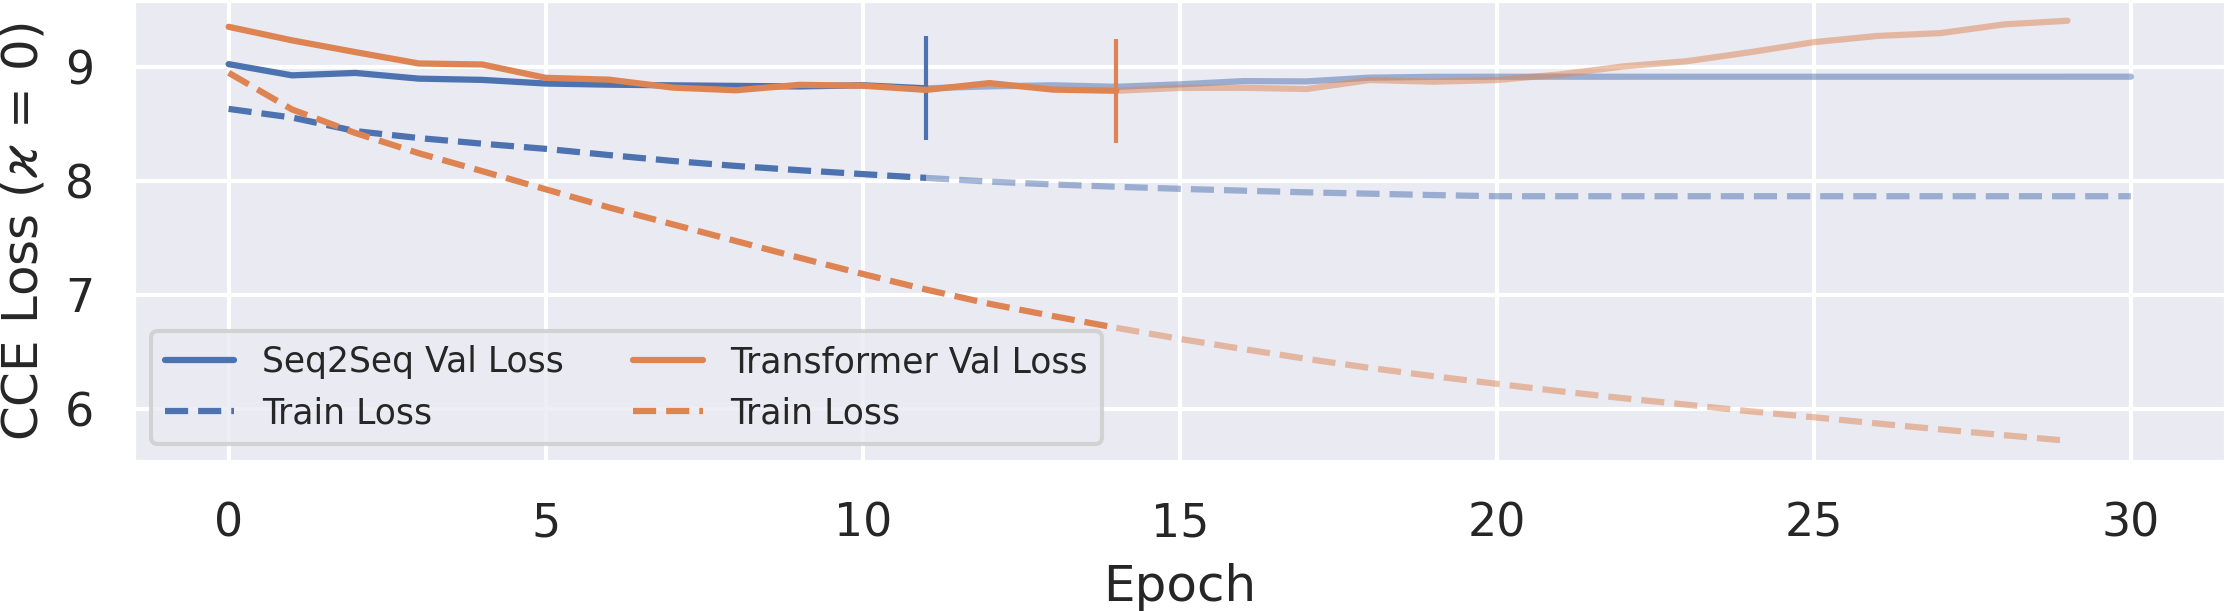
\includegraphics[width = \textwidth]{baseline_losses.png}
	\caption{Training and validation losses of both initial models. Due to early stopping, only the non-transparent part is considered.}
\end{figure}

While the categorical cross-entropy loss of these models seems similar, their ROUGE scores tell another story.
\Cref{baseline_rouges} contains the ROUGE1 and ROUGE2 scores of both models, where the transformer produces a considerably better score.

\begin{figure}[h]
	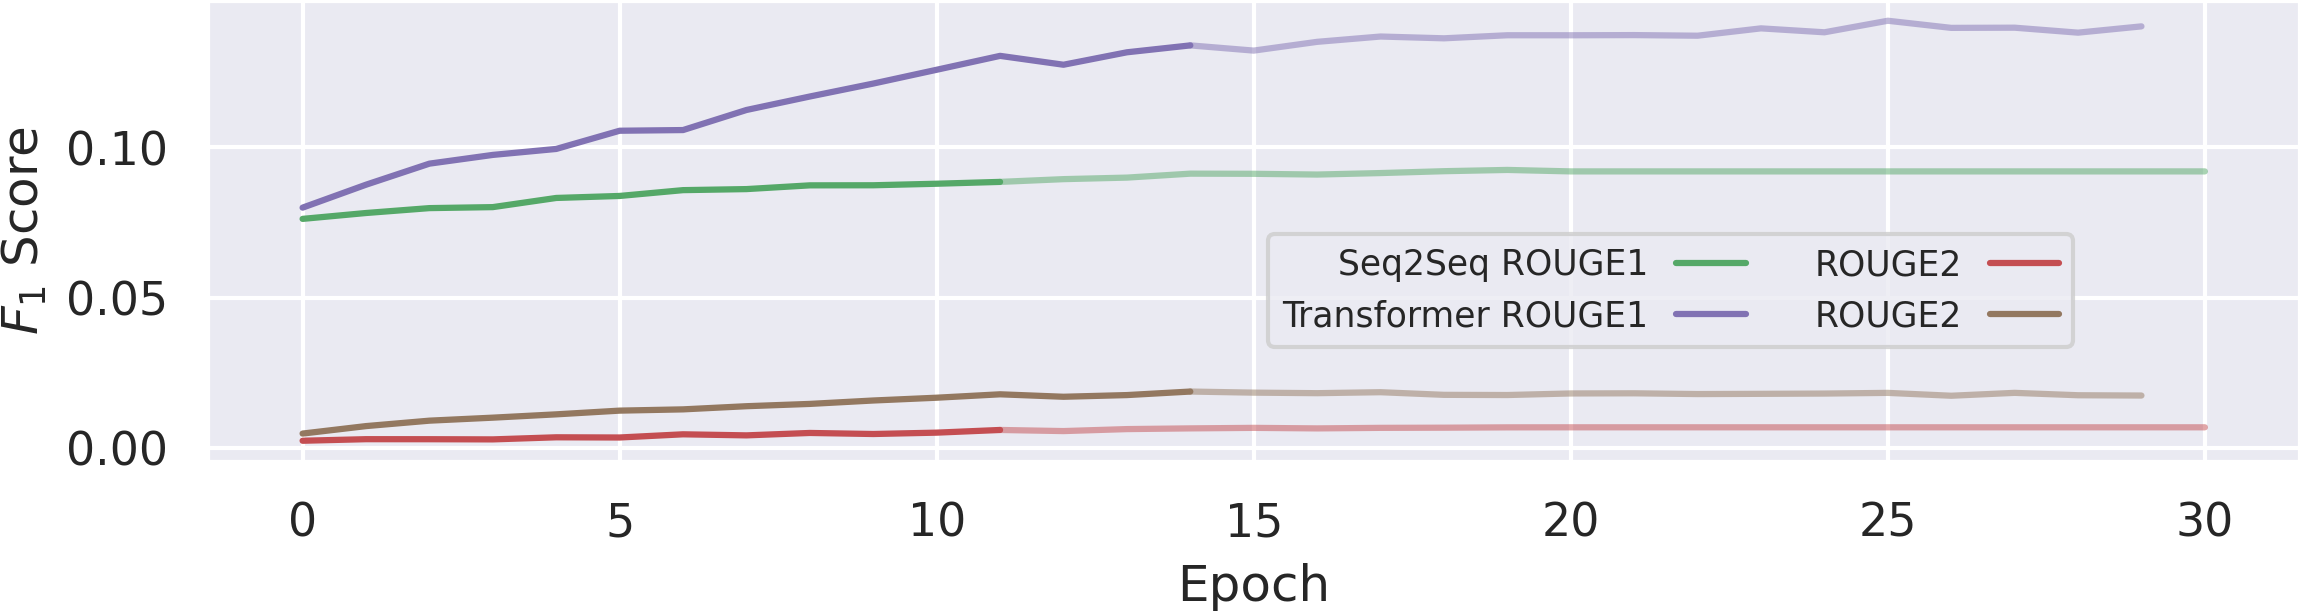
\includegraphics[width = \textwidth]{baseline_rouges.png}
	\caption{ROUGE scores of the Seq2Seq and Transformer models. The attention mechanism allows the transformer model to create more coherent result with higher ROUGE scores.}
	\label{baseline_rouges}
\end{figure}

Are these relatively good ROUGE scores good for having reasonable results?
The answer is a resounding \textbf{NO}.

\Cref{seq2seq_example,transformer_example} in \appendixA show some examples of the outputs from this model.
The results are nonsensical, and there is nothing that could even suggest where to start.
